
% --------------------------------------------------------------
\begin{frame}[fragile]
  \frametitle{PyRK: Python for Reactor Kinetics}
  \begin{itemize}
    \item 6-precursor-group, 11-decay-group PRKE model
    \item Lumped Parameter thermal hydraulics model
    \item Object-oriented, geometry and material agnostic framework
  \end{itemize}
\end{frame}


% --------------------------------------------------------------
\begin{frame}[fragile]
  \frametitle{PB-FHR RIA}
The algebraic model relies on accurate initial temperatures.
A steady state analysis with PyRK gives initial temperatures.
  \begin{figure}[htbp!]
    \begin{center}
      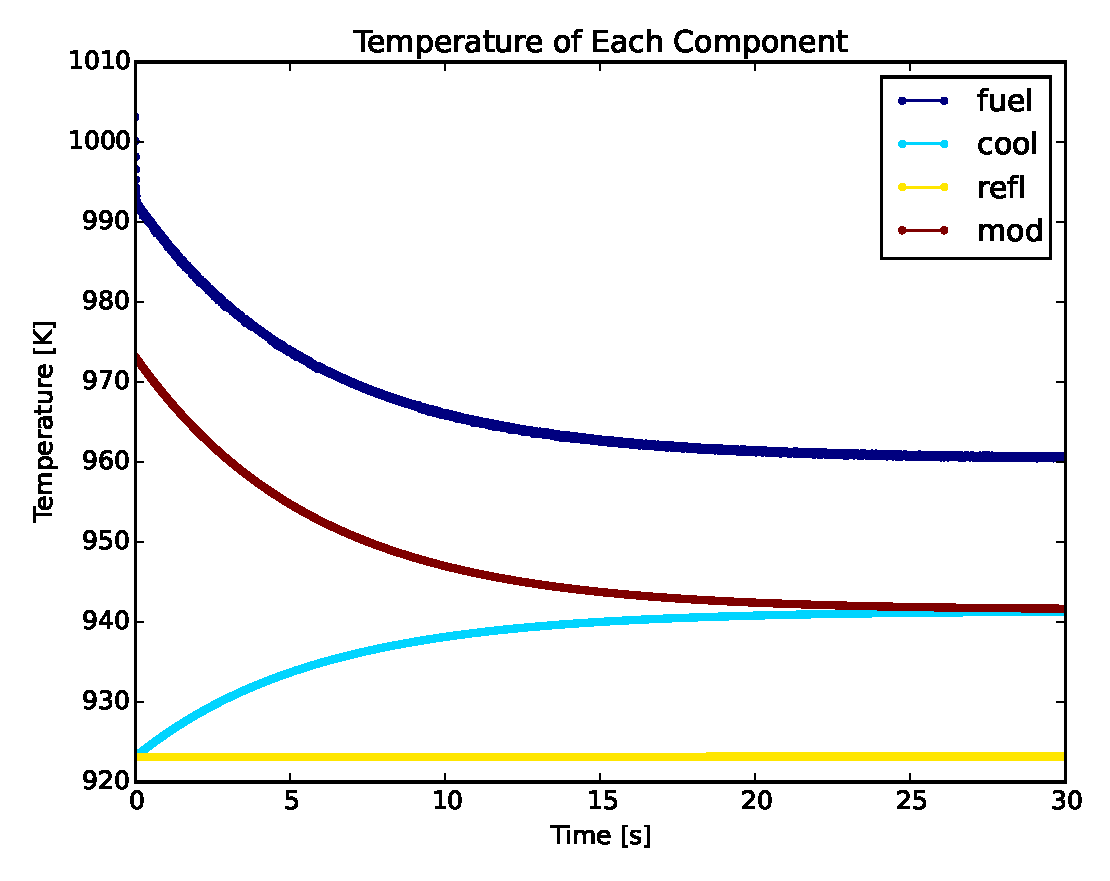
\includegraphics[height=0.7\textheight]{./progress/ss_w_o_feedbacks.eps}
    \end{center}
    \caption{Steady-State solution, four components (fuel kernels, moderating
    graphite, reflectors, and coolant).}
    \label{fig:ss_w_o_feedbacks}
  \end{figure}
\end{frame}

% --------------------------------------------------------------
\begin{frame}[fragile]
  \frametitle{PB-FHR RIA}
However, this model relies on accurate initial temperatures. A steady state
analysis with PyRK gives initial temperatures of:
\begin{align}
T_{fuel} &= 952.49 K &= 679.34 ^\circ C\\
T_{cool} &= 941.26 K &= 668.11 ^\circ C\\
T_{refl} &= 923.20 K &= 650.05 ^\circ C\\
T_{mod} &= 941.54 K  &= 668.39 ^\circ C
\end{align}

Using these temperatures, allow T to be the asymptotic temperature of the whole
system. For an insertion of $\rho$ :
\begin{align}
-\rho =& (T-679.34)\times(-3.8)+(T-668.11)\times(-1.8)\\
+&(T-650.05)\times(1.8)+(T-668.39)\times(-0.7)
\end{align}

\end{frame}
% --------------------------------------------------------------
\begin{frame}[fragile]
  \frametitle{PB-FHR RIA}
  \begin{figure}[htbp!]
    \begin{center}
      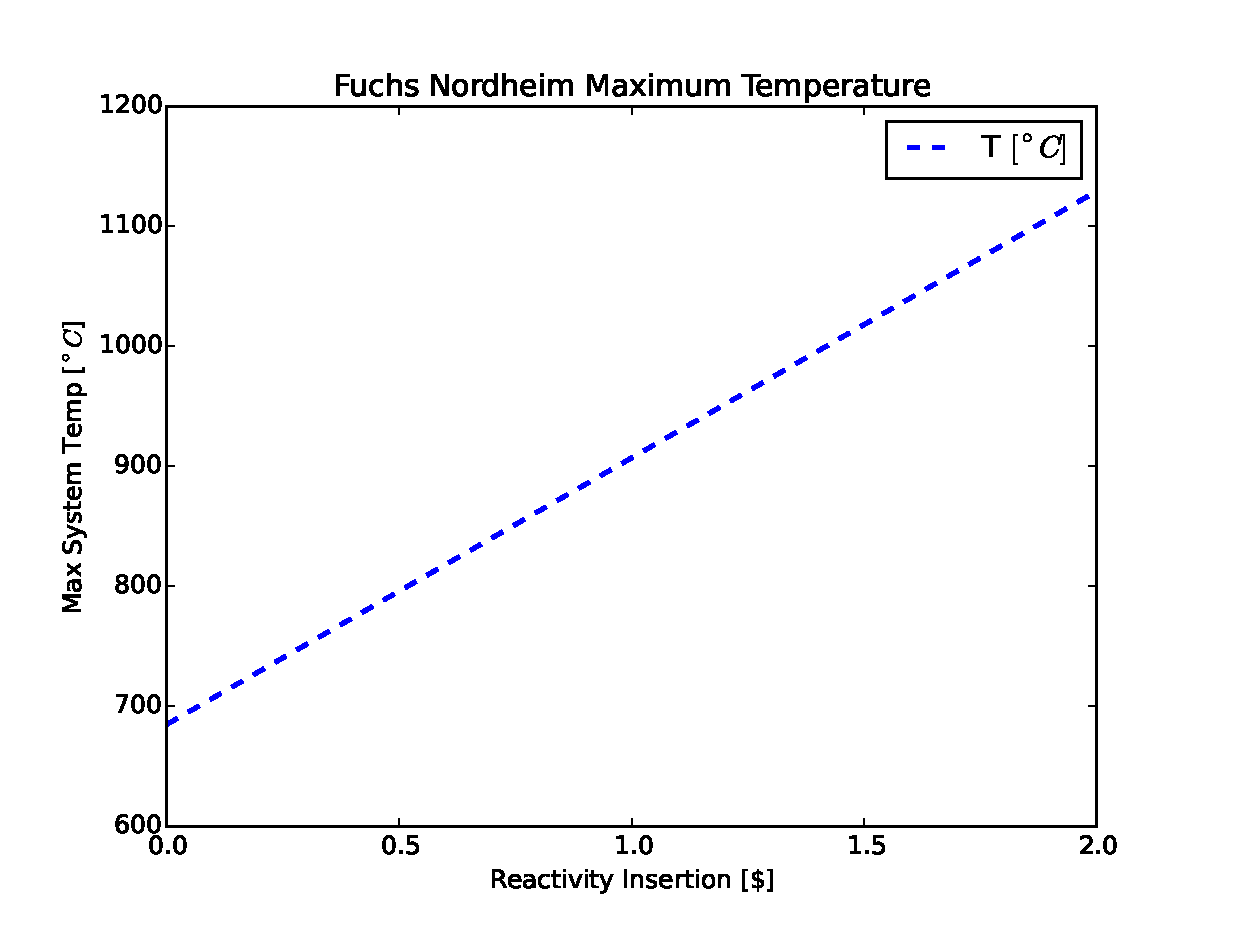
\includegraphics[height=0.7\textheight]{./progress/fn.eps}
    \end{center}
    \caption{Maximum temperature predicted by Fuchs-Nordheim based on initial
    temperatures calculated with PyRK.}
    \label{fig:fn}
  \end{figure}
\end{frame}


% --------------------------------------------------------------
\begin{frame}[fragile]
  \frametitle{Quality Control}
  \begin{itemize}
    \item Unit Checking: Pint (github.com/pint)
    \item Version Control: Git & GitHub (github.com/pyrk/pyrk)
    \item Automated Documentation: Sphinx (pyrk.github.io)
    \item Test Suite: nose
    \item Continuous Integration: Travis (travis-ci.org/pyrk/pyrk)
    \item Plotting: Matplotlib
    \item ODE solves: SciPy
  \end{itemize}
\end{frame}

% --------------------------------------------------------------
\begin{frame}[fragile]
  \frametitle{Unit Checking}
  \begin{figure}[htbp!]
    \begin{center}
      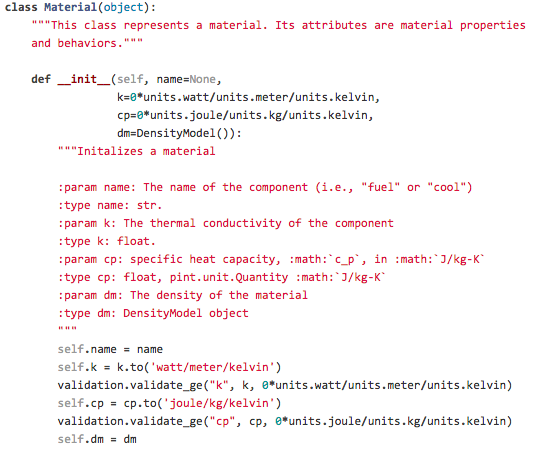
\includegraphics[height=0.7\textheight]{./progress/pint_pyrk.png}
    \end{center}
    \caption{In PyRK, the Pint package (pint.readthedocs.org/en/0.6/) is used
    keeping track of units, converting between them, and throwing errors when
    unit conversversions are not sane.}
    \label{fig:doc_pyrk}
  \end{figure}
\end{frame}
% --------------------------------------------------------------
\begin{frame}[fragile]
  \frametitle{Version Control}
  \begin{figure}[htbp!]
    \begin{center}
      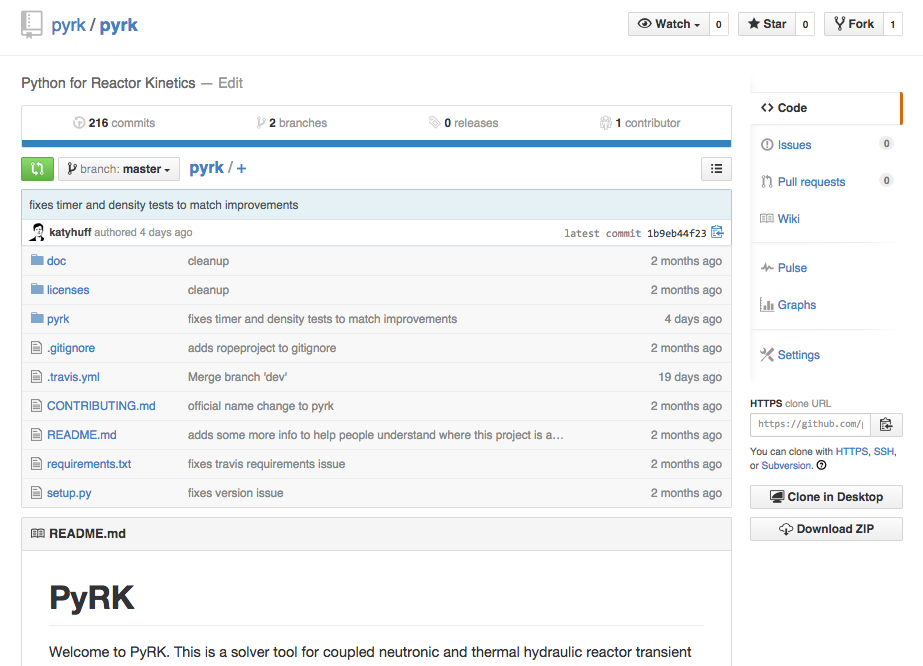
\includegraphics[height=0.7\textheight]{./progress/github_pyrk.png}
    \end{center}
    \caption{Keeping track of versions of the code makes it possible to
    experiment without fear and placing the code online encourages use and
    collaboration.}
    \label{fig:doc_pyrk}
  \end{figure}
\end{frame}

% --------------------------------------------------------------
\begin{frame}[fragile]
  \frametitle{Automated Documentation}
  \begin{figure}[htbp!]
    \begin{center}
      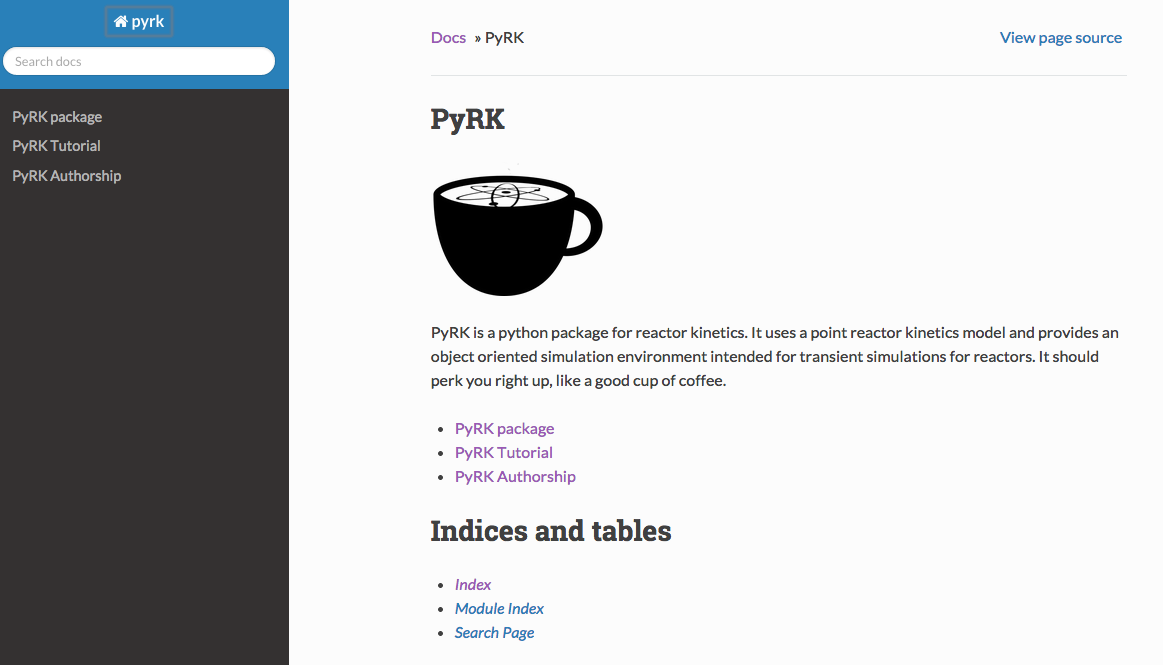
\includegraphics[height=0.7\textheight]{./progress/doc_pyrk.png}
    \end{center}
    \caption{Automated documentation creates a browsable website explaining the most recent version of the code.}
    \label{fig:doc_pyrk}
  \end{figure}
\end{frame}

% --------------------------------------------------------------
\begin{frame}[fragile]
  \frametitle{Automated Documentation}
  \begin{figure}[htbp!]
    \begin{center}
      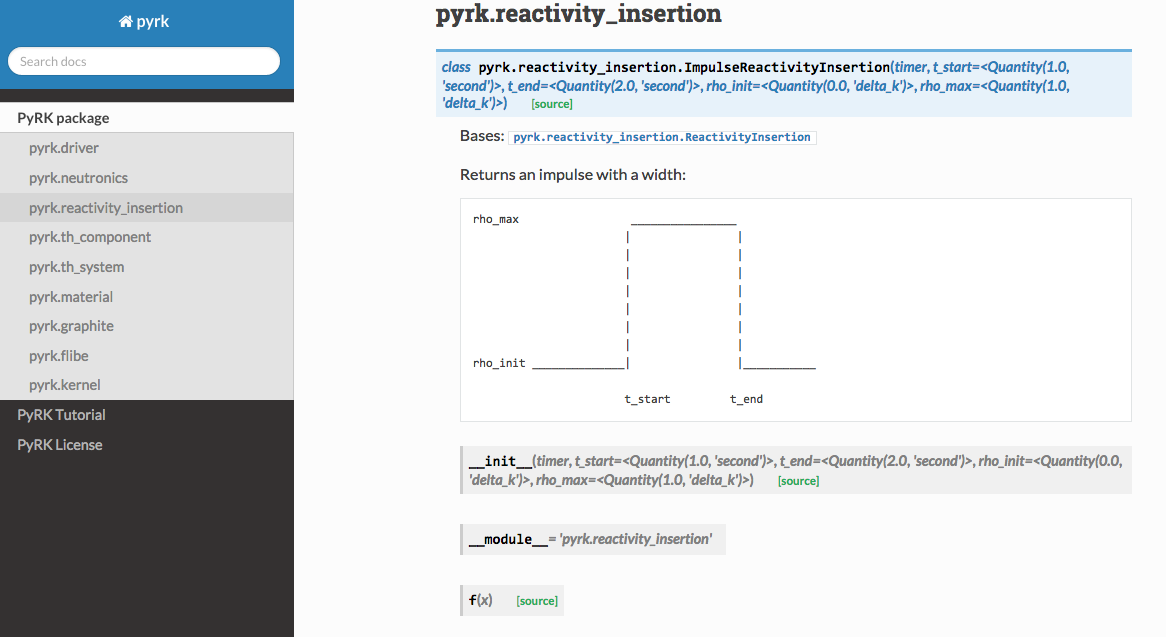
\includegraphics[width=0.9\textwidth]{./progress/doc_ri.png}
    \end{center}
    \caption{Specifically formatted comments in the code become readable,
    clickable user/developer guide.}
    \label{fig:doc_ri}
  \end{figure}
\end{frame}

% --------------------------------------------------------------
\begin{frame}[fragile]
  \frametitle{Test Suite}
  \begin{figure}[htbp!]
    \begin{center}
      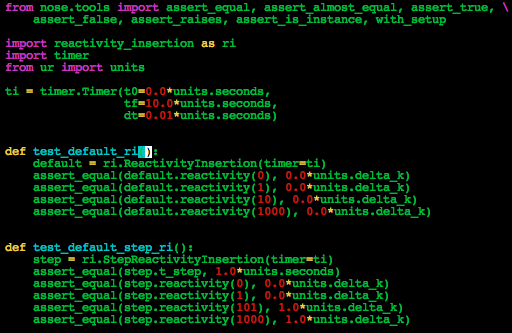
\includegraphics[height=0.7\textheight]{./progress/tests_pyrk.png}
    \end{center}
    \caption{The classes and functions that make up the code are tested individually for
   robustness.}
    \label{fig:tests_pyrk}
  \end{figure}
\end{frame}

% --------------------------------------------------------------
\begin{frame}[fragile]
  \frametitle{Continuous Integration}
  \begin{figure}[htbp!]
    \begin{center}
    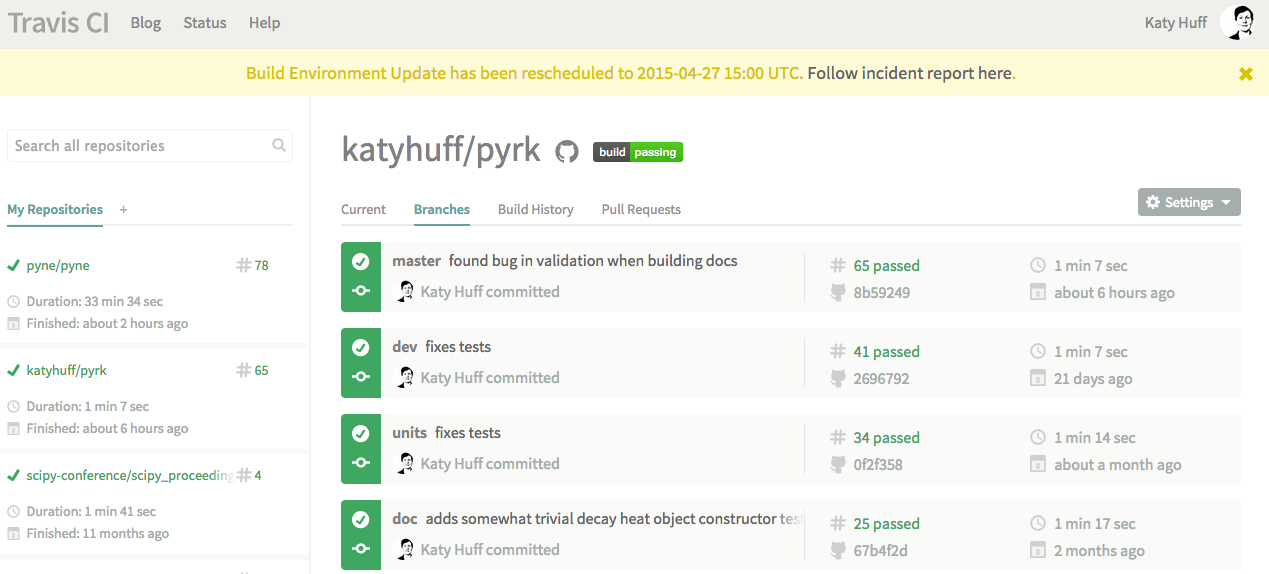
\includegraphics[height=0.6\textheight]{./progress/travis_pyrk.png}
    \end{center}
    \caption{The tests are run every time a change is made to the repository
    online. The results are public. If a main branch has a failed test, I get
    an email.}
    \label{fig:tests_pyrk}
  \end{figure}
\end{frame}

% --------------------------------------------------------------
\begin{frame}[fragile]
\frametitle{PyRK: Design}
\footnotesize{
PyRK is object oriented and modular. The important object classes in PyRK are:
\begin{itemize}
\item \textbf{SimInfo} Reads the input file, manages the solution matrix, Timer, and communication between neutronics and thermal hydraulics.
\item \textbf{Neutronics} : calculates $dP/dt$, $d\omega_j/dt$, based on
$dT_i/dt$ and the external reactivity insertion.
\item \textbf{THSystem} : manages various THComponents, facilitates their
communication.
\item \textbf{THComponent} : Conducts lumped parameter calculation. Other
thermal models can inherit from it and replace it in the simulation.
\item \textbf{Material} : A class for defining the intensive properties of a
material ($c_p$, $\rho$, $k_{th}$). Subclasses include \textbf{Flibe,
Graphite,} and \textbf{Kernel}.
\end{itemize}
}
\end{frame}
% --------------------------------------------------------------
\begin{frame}[fragile]
  \frametitle{Neutronics : Reactivity Insertion Model}
  \begin{align}
    \rho_{ext} &= \left\{
                  \begin{array}{l}
                            \mbox{ ramp } \\
                            \mbox{ pulse } \\
                            \mbox{ prompt jump }\\
                            \mbox{ control rod drop }\\
                            \mbox{ etc. } \\
                  \end{array}
                  \right.
  \end{align}
\end{frame}

% --------------------------------------------------------------
\begin{frame}[fragile]
  \frametitle{Neutronics : Reactivity Insertion Model}
  \begin{figure}[htbp!]
    \begin{center}
      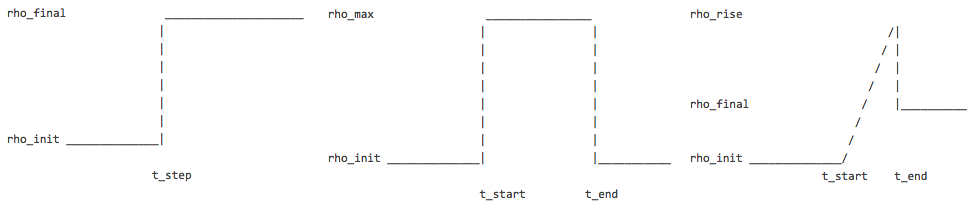
\includegraphics[width=0.95\textwidth]{./progress/ri.png}
    \end{center}
    \caption{The reactivity insertion that drives the simulator can be selected
    and customized from three models.  }
    \label{fig:ri}
  \end{figure}

\end{frame}

% --------------------------------------------------------------
\begin{frame}[fragile]
  \frametitle{Thermal Hydraulics System}
  \footnotesize{
  \begin{equation}
  \frac{d}{dt}\left[
    \begin{array}{c}
      T_{fuel} \\
      T_{cool} \\
      T_{mod} \\
      T_{refl} \\
    \end{array}
    \right]
    =
    \left[
      \begin{array}{ r }
        f(p, C_p^{fuel}, \rho_{fuel}, T_{fuel}, C_p^{cool}, v_{cool}, T_{cool},\\
          C_p^{mod}, T_{mod}, A_{fuel}, A_{mod}, \cdots )\\
          \\
        g(C_p^{fuel}, \rho_{fuel}, T_{fuel}, C_p^{cool}, v_{cool}, \rho_{cool},\\
          T_{cool}, A_{fuel}, \cdots )\\
          \\
        m(C_p^{fuel}, \rho_{fuel}, T_{fuel}, C_p^{cool}, v_{cool}, \rho_{cool},T_{cool},\\
         C_p^{mod}, \rho_{mod}, T_{mod}, A_{fuel}, A_{mod}, \cdots )\\
        \\
        r(C_p^{fuel}, \rho_{fuel}, T_{fuel}, C_p^{cool}, v_{cool}, \rho_{cool}, T_{cool},\\
         C_p^{mod}, \rho_{mod}, T_{mod}, A_{fuel}, A_{mod}, \cdots )\\
      \end{array}
      \right]
      \label{eqn:th_prke_fuller}
    \end{equation}

  }
\end{frame}


% --------------------------------------------------------------
\begin{frame}[fragile]
  \frametitle{Lumped Parameter Heat Transfer}
\footnotesize{
The heat flow out of body $i$ is the sum of surface heat flow by conduction,
convection, radiaion, and other mechanisms to each adjacent body, $j$:

\begin{align}
Q &= Q_i + \sum_j Q_{ij}\\
  &=Q_i +  \sum_j\frac{T_{i} - T_{j}}{R_{th,ij}}
\label{resistance}
\intertext{where}
\dot{Q} &= \mbox{total heat flow out of body i }[J\cdot s^{-1}]\\
Q_i &= \mbox{other heat transfer, a constant }[J\cdot s^{-1}]\\
T_i &= \mbox{temperature of body i }[K]\\
T_j &= \mbox{temperature of body j }[K]\\
j &= \mbox{adjacent bodies }[-]\\
R_{th} &= \mbox{thermal resistence of the component }[K \cdot s \cdot J^{-1}].
\end{align}
}
\end{frame}

% --------------------------------------------------------------
\begin{frame}[fragile]
  \frametitle{Lumped Parameter Heat Transfer}


\begin{table}
\centering
\begin{tabular}{|l|c|c|}
\hline
Transfer Mode & Rate of Heat Transfer & Thermal Resistance \\
\hline
Conduction
& $\dot{Q}= \frac{T_1-T_2}{\left ( \frac{L}{kA} \right )}$
& $\frac{L}{kA}$\\
\hline
Convection
&$\dot{Q}=\frac{T_{surf}-T_{envr}}{\left ( \frac{1}{h_{conv}A_{surf}} \right )}$
&$\frac{1}{h_{conv}A_{surf}}$\\
\hline
Advection
&$\dot{Q}=\frac{T_{in}-T_{out}}{\left( \frac{1}{\dot{m}c_p} \right)}$
&$\frac{1}{\dot{m}c_p}$\\
\hline
Radiation
&$\dot{Q}=\frac{T_{surf}-T_{surr}}{\left ( \frac{1}{h_rA_{surf}} \right )}$
&$\frac{1}{h_rA}$\\
\hline
\end{tabular}
\caption{Lumped Capacitance for various heat transfer modes
\cite{wikipedia_lumped_2014}.}
\label{tab:lumpedcap}
\end{table}



\end{frame}

% --------------------------------------------------------------
\begin{frame}[fragile]
  \frametitle{Lumped Parameter Heat Transfer}
\footnotesize{
  \begin{align}
    \frac{dT_{fuel}}{dT} &=  - dT_{cond,cool} - dT_{cond,mod} - dT_{conv,cool} + dT+{fission}\\
    \frac{dT_{cool}}{dT} &=  + dT_{conv,mod} - dT_{conv,refl} \\
    \frac{dT_{mod}}{dT}  &=  + dT_{cond,fuel}\\
    \frac{dT_{refl}}{dT} &=  + dT_{cond,cool}
  \end{align}
}
\end{frame}


% --------------------------------------------------------------
\begin{frame}[fragile]
\frametitle{Lumped Parameter Heat Transfer}
\footnotesize{
\begin{align}
\frac{dT_{F}}{dt} &= \frac{-\left[\frac{T_{F} - T_{M}}{R_{th,FM}} +
\frac{T_{F}-T_{S}}{R_{th,FS}}\right] + p}{\left(\rho c_pV\right)_{F}}.
\label{dTfdt}
\end{align}

Here, the surface area between the matrix graphite and the fuel is the set of
$N_pN_T$ shells of radius $r_T$.  Additionally, the volume is the sum of
$N_PN_T$ spherical volumes of radius $r_T$.

\begin{align}
R_{th,FM} &= \frac{r_F}{k_FA_{FM}}\\
          &= \frac{r_F}{4\pi N_pr_M^2k_F}\\
          &= \frac{1}{4\pi N_pr_Mk_F}\\
R_{th,FS} &= \frac{r_F}{k_FA_{FS}}\\
          &= \frac{r_F}{4\pi N_pr_S^2k_F}\\
          &= \frac{1}{4\pi N_pr_Sk_F}
\end{align}
}
\end{frame}



% --------------------------------------------------------------
\begin{frame}[fragile]
\frametitle{Adding Components}
  \begin{figure}[htbp!]
    \begin{center}
      \includegraphics[height=0.7\textheight]{./progress/add_components.png}
    \end{center}
    \caption{Components are added in the input file and rely on the available
    (small) library of material classes.}
    \label{fig:ss_w_o_feedbacks}
  \end{figure}
\end{frame}

% --------------------------------------------------------------
\begin{frame}[fragile]
\frametitle{Connecting Components}
  \begin{figure}[htbp!]
    \begin{center}
      \includegraphics[height=0.7\textheight]{./progress/add_interfaces.png}
    \end{center}
    \caption{Connections between thermal components are added in the input
    file.}
    \label{fig:ss_w_o_feedbacks}
  \end{figure}
\end{frame}



% --------------------------------------------------------------
\begin{frame}[fragile]
\frametitle{Running a Steady State Simulation}
\input{./pebble/pebble_components}
\end{frame}

% --------------------------------------------------------------
\begin{frame}[fragile]
\frametitle{Running a Steady State Simulation}
  \begin{figure}[htbp!]
    \begin{center}
      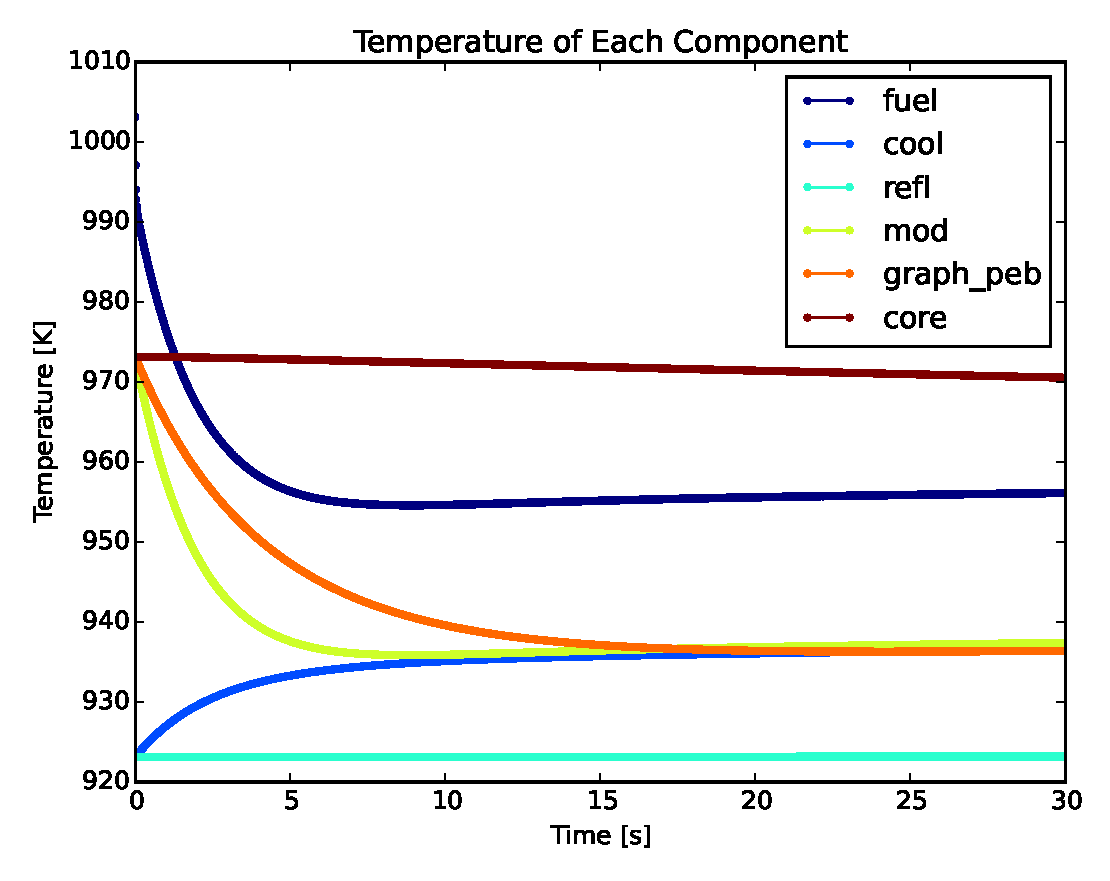
\includegraphics[height=0.7\textheight]{./progress/temps_all_comps_ss.eps}
    \end{center}
    \caption{Steady-State solution, four components (fuel kernels, moderating
    graphite, reflectors, and coolant).}
    \label{fig:ss_w_o_feedbacks}
  \end{figure}
\end{frame}

% --------------------------------------------------------------
\begin{frame}[fragile]
\frametitle{Running a Positive Step Insertion Simulation}
  \begin{figure}[htbp!]
    \begin{center}
      \includegraphics[height=0.7\textheight]{./progress/coupled_t_fb_001_pow_rho.eps}
    \end{center}
    \caption{Step reactivity insertion of 0.001 $\Delta k$ at 1 s, six components (fuel kernels, moderating graphite annulus, moderating graphite core, reflector pebbles, reflectors, and coolant).}
    \label{fig:all_comps_temps}
  \end{figure}
\end{frame}
% --------------------------------------------------------------
\begin{frame}[fragile]
\frametitle{Running a Positive Step Insertion Simulation}
  \begin{figure}[htbp!]
    \begin{center}
      \includegraphics[height=0.7\textheight]{./progress/coupled_t_fb_001_temps.eps}
    \end{center}
    \caption{Step reactivity insertion of 0.001 $\Delta k$ at 1 s, six components (fuel kernels, moderating graphite annulus, moderating graphite core, reflector pebbles, reflectors, and coolant).}
    \label{fig:all_comps_temps}
  \end{figure}
\end{frame}


% --------------------------------------------------------------
\begin{frame}[fragile]
\frametitle{Running a Negative Step Insertion Simulation}
  \begin{figure}[htbp!]
    \begin{center}
      \includegraphics[height=0.7\textheight]{./progress/neg_01_pow_rho.eps}
    \end{center}
    \caption{Negative step reactivity insertion of 0.01 $\Delta k$ at 1 s, six components (fuel kernels, moderating graphite annulus, moderating graphite core, reflector pebbles, reflectors, and coolant).}
    \label{fig:all_comps_temps}
  \end{figure}
\end{frame}

% --------------------------------------------------------------
\begin{frame}[fragile]
\frametitle{Running a Negative Step Insertion Simulation}
  \begin{figure}[htbp!]
    \begin{center}
      \includegraphics[height=0.7\textheight]{./progress/neg_01_fuel_temp.eps}
    \end{center}
    \caption{Negative step reactivity insertion of 0.01 $\Delta k$ at 1 s, six components (fuel kernels, moderating graphite annulus, moderating graphite core, reflector pebbles, reflectors, and coolant).}
    \label{fig:all_comps_temps}
  \end{figure}
\end{frame}

% --------------------------------------------------------------
\begin{frame}[fragile]
\frametitle{Running a Negative Step Insertion Simulation}
  \begin{figure}[htbp!]
    \begin{center}
      \includegraphics[height=0.7\textheight]{./progress/neg_01_zetas.eps}
    \end{center}
    \caption{Negative step reactivity insertion of 0.01 $\Delta k$ at 1 s, six components (fuel kernels, moderating graphite annulus, moderating graphite core, reflector pebbles, reflectors, and coolant).}
    \label{fig:all_comps_temps}
  \end{figure}
\end{frame}


% --------------------------------------------------------------
\begin{frame}[fragile]
\frametitle{Running a Positive Impulse Insertion Simulation}
  \begin{figure}[htbp!]
    \begin{center}
      \includegraphics[height=0.7\textheight]{./progress/coupled_001_impulse_rho.eps}
    \end{center}
    \caption{Positive pulse reactivity insertion of 0.001 $\Delta k$ at 1 s, six components (fuel kernels, moderating graphite annulus, moderating graphite core, reflector pebbles, reflectors, and coolant).}
    \label{fig:all_comps_temps}
  \end{figure}
\end{frame}


% --------------------------------------------------------------
\begin{frame}[fragile]
\frametitle{Running a Positive Impulse Insertion Simulation}
  \begin{figure}[htbp!]
    \begin{center}
      \includegraphics[height=0.7\textheight]{./progress/coupled_001_impulse_pow_and_rho.eps}
    \end{center}
    \caption{Positive pulse reactivity insertion of 0.001 $\Delta k$ at 1 s, six components (fuel kernels, moderating graphite annulus, moderating graphite core, reflector pebbles, reflectors, and coolant).}
    \label{fig:all_comps_temps}
  \end{figure}
\end{frame}


% --------------------------------------------------------------
\begin{frame}[fragile]
\frametitle{Running a Positive Impulse Insertion Simulation}
  \begin{figure}[htbp!]
    \begin{center}
      \includegraphics[height=0.7\textheight]{./progress/coupled_001_impulse_temps.eps}
    \end{center}
    \caption{Positive pulse reactivity insertion of 0.001 $\Delta k$ at 1 s, six components (fuel kernels, moderating graphite annulus, moderating graphite core, reflector pebbles, reflectors, and coolant).}
    \label{fig:all_comps_temps}
  \end{figure}
\end{frame}


